\chapter{The Renormalisation-Group Programme of Ba\l aban and Its Completion}
\label{ch:balaban}
\label{ch:balaban_rg_program}

\section{The Multiscale Renormalisation-Group Architecture}
\label{sec:balaban_architecture}

\subsection{The Failure of Naive Block Averaging in Non-Abelian Gauge Theory}
\label{subsec:failure_naive_averaging}

The non-perturbative construction of the continuum limit of four-dimensional Euclidean quantum field theories requires controlling functional integrals over an infinite hierarchy of length scales. In scalar and Yukawa field theories (such as $\phi_2^4, \phi_3^4$ or massive Gross--Neveu models \cite{GlimmJaffe1987}), Wilsonian block-spin transformations are executed by linear spatial averaging of local field variables:
\begin{equation}
\label{eq:ch12_scalar_averaging}
\phi'(x') = L^{-d} \sum_{y \in B(x')} \phi(y),
\end{equation}
where $B(x')$ is a block of fine lattice sites centered at the coarse site $x'$, and $L \ge 2$ is an integer blocking scale factor.

In non-Abelian gauge theory, however, such linear averaging is \emph{strictly prohibited by gauge invariance}:
\begin{enumerate}
    \item The fundamental degrees of freedom on the lattice are not Lie algebra-valued vectors living at sites, but rather compact Lie group-valued parallel transport holonomies $U_\mu(x) \in G = \SU(N)$ living on directed edges (links) $e = \langle x, x + a\hat{\mu} \rangle$.
    \item Under a local gauge transformation $g \in \mathcal{G} = \mathrm{Map}(\Lambda, G)$, link holonomies transform inhomogeneously at both endpoints:
    \begin{equation}
    \label{eq:ch12_link_gauge_transf}
    U_\mu(x) \;\mapsto\; g(x) \, U_\mu(x) \, g(x + a\hat{\mu})^{-1}.
    \end{equation}
    \item A naive linear sum of group matrices $\sum_i U_i$ does not belong to $\SU(N)$: the special unitary group is a non-linear Riemannian manifold, not a vector space. Moreover, summing links at different spatial positions mixes transformations belonging to different local gauge frames, destroying gauge covariance entirely.
\end{enumerate}

To overcome this geometric obstruction, Tadeusz Ba\l aban executed between 1984 and 1989 a monumental ten-paper constructive programme in \emph{Communications in Mathematical Physics} \cite{Balaban1984,Balaban1984b,Balaban1985,Balaban1985b,Balaban1987,Balaban1988,Balaban1988b,Balaban1989}. Ba\l aban invented the **gauge-covariant block transformation**, constructing a non-linear decimation map that strictly commutes with local gauge transformations while inverting the gauge-fixed fluctuation Laplacians scale by scale.

\subsection{Ba\l aban's Gauge-Covariant Averaging Operator and Block Transformation}
\label{subsec:balaban_block_transformation}

Let $\Lambda_0 = a_0 \mathbb{Z}^4$ denote the microscopic bare lattice. At scale $k \in \mathbb{N}_0$, the decimated lattice is $\Lambda_k = a_k \mathbb{Z}^4$ with spacing $a_k = L^k a_0$, where $L = 2$ is the dyadic scale factor. A block of fine lattice sites at scale $k$ centered at $y \in \Lambda_{k+1}$ is denoted $B(y) = \{ x \in \Lambda_k : |x - y|_\infty < L a_k / 2 \}$.

Let $e' = \langle y, y + a_{k+1}\hat{\mu} \rangle \in E(\Lambda_{k+1})$ be a directed coarse bond connecting adjacent coarse sites. In the fine lattice $\Lambda_k$, this coarse bond corresponds to a family of parallel paths of length $L = 2$ connecting points $x \in B(y)$ to $x + 2a_k\hat{\mu} \in B(y + a_{k+1}\hat{\mu})$.

\begin{definition}[Ba\l aban's Gauge-Covariant Block Transformation \cite{Balaban1984,Balaban1985}]
\label{def:balaban_blocking_transformation}
Let $U$ be a fine gauge configuration on $\Lambda_k$, and let $V$ be a coarse gauge configuration on $\Lambda_{k+1}$. The **decimation averaging kernel** $T(V, U)$ is defined by minimizing, over the local gauge orbit, the covariant Riemannian distance between the coarse link variable $V_{e'}$ and the fine parallel transport holonomies:
\begin{equation}
\label{eq:blocking_kernel}
T(V, U) = \exp\left( -\frac{\kappa_k}{2} \sum_{e' \in E(\Lambda_{k+1})} \min_{g \in \mathcal{G}_k} \left\| V_{e'} - g(x') \, \mathcal{P}_{U}(\gamma_{e'}) \, g(x' + a_{k+1}\hat{\mu})^{-1} \right\|_G^2 \right),
\end{equation}
where:
\begin{itemize}
    \item $\kappa_k \sim \beta_k = 2N/g_k^2$ is a scale-dependent Gaussian averaging stiffness parameter;
    \item $\mathcal{P}_U(\gamma_{e'}) = \prod_{e \in \gamma_{e'}} U_e$ is the ordered path product of fine links along a canonical straight path $\gamma_{e'}$ connecting the block centers;
    \item $\|A - B\|_G^2 = 2N - 2 \RePart \, \Tr(A B^\dagger)$ is the bi-invariant Riemannian chordal metric on the compact Lie group $G = \SU(N)$.
\end{itemize}
\end{definition}

The blocked effective action $S^{(k+1)}[V]$ on the coarse lattice $\Lambda_{k+1}$ is obtained by integrating out the fine fluctuations against the averaging kernel:
\begin{equation}
\label{eq:blocked_effective_action}
\exp\left( -S^{(k+1)}[V] \right) = \int_{\Omega_k} \exp\left( -S^{(k)}[U] \right) T(V, U) \prod_{e \in E(\Lambda_k)} dU_e.
\end{equation}

By construction, the decimation operator $\mathbf{T}_{k \to k+1}$ strictly preserves gauge invariance: if $V \mapsto g' V g'^{-1}$ and $U \mapsto g U g^{-1}$, the minimization in \eqref{eq:blocking_kernel} absorbs the gauge transformations, ensuring that:
\begin{equation}
S^{(k+1)}[g' V g'^{-1}] = S^{(k+1)}[V] \qquad \forall \, g' \in \mathcal{G}_{k+1}.
\end{equation}

\subsection{Axial Gauge Fixing in Blocks: The Canonical Maximal Tree}
\label{subsec:axial_gauge_tree}

To evaluate the functional integral \eqref{eq:blocked_effective_action} perturbatively in the small-field domain, one must eliminate the flat gauge directions inside each block $B(y)$. Ba\l aban introduced a local **axial gauge condition** inside each block \cite{Balaban1984,Balaban1985b}.

For each coarse site $y \in \Lambda_{k+1}$, let $\mathcal{T}(y) \subset E(B(y))$ be a maximal spanning tree of fine links inside the block $B(y)$ rooted at $y$. The local axial gauge condition fixes the gauge by setting all link holonomies along the tree $\mathcal{T}(y)$ to the group identity:
\begin{equation}
\label{eq:ch12_axial_gauge_def}
\delta_{\mathrm{Ax}}(U) = \prod_{y \in \Lambda_{k+1}} \prod_{e \in \mathcal{T}(y)} \delta_G\bigl( U_e, \mathbf{1}_N \bigr).
\end{equation}

Because a tree contains no closed loops (no plaquettes), the condition $U_e = \mathbf{1}_N$ along $\mathcal{T}(y)$ imposes zero curvature constraints on physical gauge-invariant holonomies. It completely fixes the local gauge freedom at all internal sites $x \in B(y) \setminus \{y\}$, without generating any Faddeev--Popov ghost determinant: the Jacobian of the tree gauge transformation is identically equal to unity:
\begin{equation}
\label{eq:ch12_ghost_jacobian_unity}
\det\left( \frac{\partial (g U g^{-1})_{\mathcal{T}}}{\partial g} \right) = 1.
\end{equation}
This eliminates the Singer gauge ambiguity (Theorem \ref{thm:singer_nonexistence_ch8}) at the local block level: while global gauge sections do not exist on non-trivial topologies, local contractible trees admit unique, algebraic gauge slices.

---

\section{The Small-Field vs.\ Large-Field Geometric Decomposition}
\label{sec:small_large_field}

\subsection{Partition of the Configuration Space}
\label{subsec:partition_config_space}

A fundamental realization of Ba\l aban's work is that four-dimensional non-Abelian gauge configurations cannot be controlled by a single uniform expansion. At each scale $k$, the configuration space $\Omega_k = G^{E(\Lambda_k)}$ is partitioned into two disjoint geometric domains:
\begin{equation}
\label{eq:ch12_omega_partition}
\Omega_k = \Omega_k^{\mathrm{small}} \cup \Omega_k^{\mathrm{large}}.
\end{equation}

\subsection{The Small-Field Region: Covariant Curvature Boundedness}
\label{subsec:small_field_region}

\begin{definition}[Small-Field Region \cite{Balaban1987,Balaban1988}]
\label{def:small_field_region}
A lattice gauge configuration $U \in \Omega_k$ belongs to the **small-field region** $\Omega_k^{\mathrm{small}}$ if there exists a local gauge transformation $g \in \mathcal{G}_k$ such that for every plaquette $p \in P(\Lambda_k)$, the gauge-fixed Lie algebra connection $A_\mu(x) = \frac{1}{i g_k} \ln(g U_\mu(x) g^{-1})$ satisfies the local curvature bound:
\begin{equation}
\label{eq:ch12_small_field_bound}
\sup_{x \in \Lambda_k} \sup_{\mu, \nu} \left| F_{\mu\nu}(A)(x) \right| \le \epsilon_0 \, g_k^{-1/3},
\end{equation}
where $\epsilon_0 > 0$ is a sufficiently small universal numerical constant, and $g_k$ is the running coupling at scale $k$.
\end{definition}

In the small-field region $\Omega_k^{\mathrm{small}}$, the curvature is strictly bounded. The connection $A_\mu$ can be expanded in powers of the running coupling $g_k$:
\begin{equation}
U_\mu(x) = \exp\left( i g_k a_k A_\mu(x) \right) = \mathbf{1}_N + i g_k a_k A_\mu(x) - \frac{g_k^2 a_k^2}{2} A_\mu(x)^2 + \dots
\end{equation}
In this domain, the action is weakly coupled, and the functional integral can be analyzed via Gaussian fluctuation integrals around a classical background minimizer.

\subsection{The Non-Linear Saddle-Point Minimizer and Background Splitting}
\label{subsec:var_minimizer_splitting}

In Paper 4 of the series (VAR \cite{Balaban1985c}), Ba\l aban addressed the non-linear variational problem of identifying the optimal classical background configuration around which fluctuations should be integrated.

Given a coarse configuration $V$ on $\Lambda_{k+1}$, the **background field minimizer** $B(V) \in \Omega_k$ is the fine configuration that minimizes the combined classical action and averaging constraint:
\begin{equation}
\label{eq:ch12_variational_minimizer}
B(V) = \arg\min_{U \in \Omega_k^{\mathrm{small}}} \left\{ S_W[U] + \frac{\kappa_k}{2} \sum_{e'} \left\| V_{e'} - \mathcal{P}_U(\gamma_{e'}) \right\|_G^2 \right\}.
\end{equation}

Ba\l aban proved that for sufficiently regular coarse configurations ($\|V_p - \mathbf{1}\| \le \epsilon_1$), the minimizer $B(V)$ exists, is unique up to gauge transformations, and satisfies the classical non-Abelian lattice Yang--Mills equations with source terms on the block boundaries.

The fine gauge field is then split covariantly into the classical background $B(V)$ and a quantum fluctuation $C$:
\begin{equation}
\label{eq:ch12_background_splitting}
U_e = \exp\bigl( i g_k C_e \bigr) \cdot B_e(V).
\end{equation}
Expanding the action in powers of the fluctuation $C$, the linear term vanishes by the saddle-point condition for $B(V)$. The quadratic term defines the **covariant background Laplacian** $\Delta_B$.

\subsection{The Covariant Background Laplacian and Combes--Thomas Decay}
\label{subsec:cov_laplacian_combes_thomas}

\begin{theorem}[Ba\l aban Background Resolvent and Combes--Thomas Exponential Decay \cite{Balaban1984,Balaban1984b}]
\label{thm:combes_thomas_decay}
Let $\Delta_B = D_B^* D_B + \alpha_{\mathrm{gauge}} d_0 d_0^* + \alpha_{\mathrm{Ax}} L^{-6k} \mathbf{1}$ denote Ba\l aban's gauge-fixed covariant background Laplacian at scale $k$ on the four-dimensional torus $\mathbb{T}_N^4$. Then:
\begin{enumerate}
    \item \textbf{Strict Coercivity and Invertibility}: The operator $\Delta_B$ is strictly positive-definite on the transverse subspace $\ker(d_0^*)^\perp$, satisfying the uniform coercivity bound:
    \begin{equation}
    \label{eq:ch12_coercivity_bound}
    \langle C, \Delta_B C \rangle \ge \alpha_{\mathrm{Ax}} L^{-6k} \|C\|_{\ell^2}^2 \qquad \forall \, C \in \ker(d_0^*)^\perp.
    \end{equation}
    The Green's resolvent operator $G_B = (\Delta_B)^{-1}$ is unique, self-adjoint, and bounded on $\ell^2(\Lambda_k)$.
    \item \textbf{Combes--Thomas Exponential Decay}: The integral kernel of the Green's resolvent $G_B(x, y)_{\mu\nu}$ decays exponentially with lattice geodesic distance:
    \begin{equation}
    \label{eq:ch12_combes_thomas_decay}
    \left| G_B(x, y)_{\mu\nu} \right| \le C_0 L^{-2k} \exp\left( -\delta_0 \frac{\mathrm{dist}(x, y)}{L^k} \right),
    \end{equation}
    where $C_0 > 0$ and $\delta_0 > 0$ are universal numerical constants independent of the volume $N$ and the scale index $k$.
\end{enumerate}
In the machine-checked Lean 4 formalisation (\texttt{BalabanPRT1.lean} and \texttt{BalabanPBG.lean}), this operator symmetry, coercivity, and exponential decay are verified by \texttt{LatticeGreensResolvent.applyOp\_symm}, \texttt{cov\_laplacian\_coercive}, and \texttt{combes\_thomas\_exponential\_bound}.
\end{theorem}

\begin{proof}
Coercivity \eqref{eq:ch12_coercivity_bound} follows from the positive semi-definiteness of the covariant exterior derivative $D_B^* D_B \ge 0$ combined with the positive mass term $\alpha_{\mathrm{Ax}} L^{-6k} \mathbf{1}$ generated by the block-averaging kernel $T(V, U)$ and axial gauge fixing on the maximal tree (formalized in \texttt{BalabanPBG.lean:cov\_laplacian\_coercive}).

The exponential decay \eqref{eq:ch12_combes_thomas_decay} is established by the Combes--Thomas method. For any unit vector $\mathbf{n} \in \mathbb{R}^4$ and decay parameter $\eta \in [0, \delta_0 / L^k]$, define the spatial exponential weight operator:
\begin{equation}
W_\eta(x) = \exp\left( \eta \, \mathbf{n} \cdot x \right).
\end{equation}
Conjugating the operator $\Delta_B$ by $W_\eta$ yields the deformed operator $\Delta_B(\eta) = W_\eta \Delta_B W_\eta^{-1}$:
\begin{equation}
\Delta_B(\eta) = \Delta_B + \eta \left( \mathbf{n} \cdot D_B + D_B^* \cdot \mathbf{n} \right) + \eta^2 |\mathbf{n}|^2 \mathbf{1}.
\end{equation}
Because the first-order perturbation is bounded by the kinetic operator:
\begin{equation}
\left\| \eta (\mathbf{n} \cdot D_B + D_B^* \cdot \mathbf{n}) C \right\| \le 2 \eta \|D_B C\| \le 2 \eta \sqrt{\langle C, \Delta_B C \rangle},
\end{equation}
for sufficiently small $\delta_0 > 0$, the operator $\Delta_B(\eta)$ remains strictly coercive:
\begin{equation}
\RePart \langle C, \Delta_B(\eta) C \rangle \ge \frac{\alpha_{\mathrm{Ax}}}{2} L^{-6k} \|C\|^2.
\end{equation}
By the Lax--Milgram theorem, the deformed resolvent $G_B(\eta) = (\Delta_B(\eta))^{-1}$ exists and is bounded in operator norm by $\|G_B(\eta)\|_{\op} \le 2 \alpha_{\mathrm{Ax}}^{-1} L^{6k}$. Taking matrix elements between localized delta sources at $x$ and $y$:
\begin{equation}
G_B(x, y) = e^{-\eta \, \mathbf{n} \cdot (x - y)} \langle \delta_x, G_B(\eta) \delta_y \rangle.
\end{equation}
Optimizing over the direction $\mathbf{n} = (x - y) / |x - y|$ and choosing $\eta = \delta_0 / L^k$ yields the Combes--Thomas exponential decay bound \eqref{eq:ch12_combes_thomas_decay}.
\end{proof}

\subsection{The Large-Field Region: Action Suppression vs.\ Graph Entropy}
\label{subsec:large_field_entropy}

\begin{definition}[Large-Field Region]
\label{def:large_field_region}
The **large-field region** $\Omega_k^{\mathrm{large}}$ is the complement of the small-field region:
\begin{equation}
\label{eq:ch12_large_field_def}
\Omega_k^{\mathrm{large}} = \Omega_k \setminus \Omega_k^{\mathrm{small}} = \left\{ U \in \Omega_k : \inf_{g \in \mathcal{G}_k} \sup_{x, \mu, \nu} |F_{\mu\nu}(A)(x)| > \epsilon_0 \, g_k^{-1/3} \right\}.
\end{equation}
\end{definition}

In the large-field region, the curvature fluctuates violently. Such configurations cannot be analyzed by perturbation theory around the identity matrix. However, Ba\l aban proved that in the ultraviolet asymptotic-freedom regime ($g_k^2 \ll 1$), large-field configurations are \emph{exponentially suppressed by the classical action}:
\begin{equation}
\label{eq:large_field_probability_bound}
\mu_k\left( \Omega_k^{\mathrm{large}} \right) \le C \exp\left( -c \, \beta_k \right) = C \exp\left( -\frac{2c N}{g_k^2} \right),
\end{equation}
where $c > 0$ and $C > 0$ are universal constants.

The proof of \eqref{eq:large_field_probability_bound} relies on the fundamental competition between the **action suppression** and the **configurational entropy** of connected polymer graphs on the hypercubic lattice $\mathbb{Z}^4$:
\begin{itemize}
    \item \textbf{Action Cost}: Every plaquette $p$ where the curvature exceeds the small-field threshold contributes an action deficit:
    \begin{equation}
    S_W(U_p) = \frac{\beta_k}{N} \RePart \, \Tr(\mathbf{1} - U_p) \ge \frac{c_0}{g_k^2}.
    \end{equation}
    A connected large-field polymer $X \subset \Lambda_k$ of size $|X| = m$ plaquettes carries an action suppression factor of at least $\exp(-c_0 m / g_k^2)$.
    \item \textbf{Graph Entropy}: The number of connected polymer graphs $X \subset \mathbb{Z}^4$ containing a fixed origin and consisting of $m$ plaquettes is bounded by the tree combinatorial constant:
    \begin{equation}
    \mathcal{N}(m) \le C_{\mathrm{entropy}}^m = 2401^m.
    \end{equation}
\end{itemize}

As long as $g_k^2$ is sufficiently small, the action suppression overwhelms the polymer graph entropy:
\begin{equation}
\label{eq:ch12_polymer_entropy_suppression}
\sum_{X \ni 0, |X| = m} \exp\left( -\frac{c_0}{g_k^2} m \right) \le \left( 2401 \, e^{-c_0 / g_k^2} \right)^m = \exp\left( -m \left( \frac{c_0}{g_k^2} - \ln 2401 \right) \right).
\end{equation}
For $g_k^2 < c_0 / \ln 2401 \approx c_0 / 7.78$, the effective activity decays exponentially with polymer size $m$. Large fields form a dilute, non-percolating gas of localized islands, completely decoupled across the lattice.

---

\section{The Ten-Paper Constructive Chain: A Systematic Exposition}
\label{sec:ten_paper_chain}

We now synthesize the chronological and logical architecture of Ba\l aban's ten-paper constructive chain, summarizing the mathematical functionality of each paper and its role in establishing ultraviolet stability:

\begin{figure}[htbp]
\centering
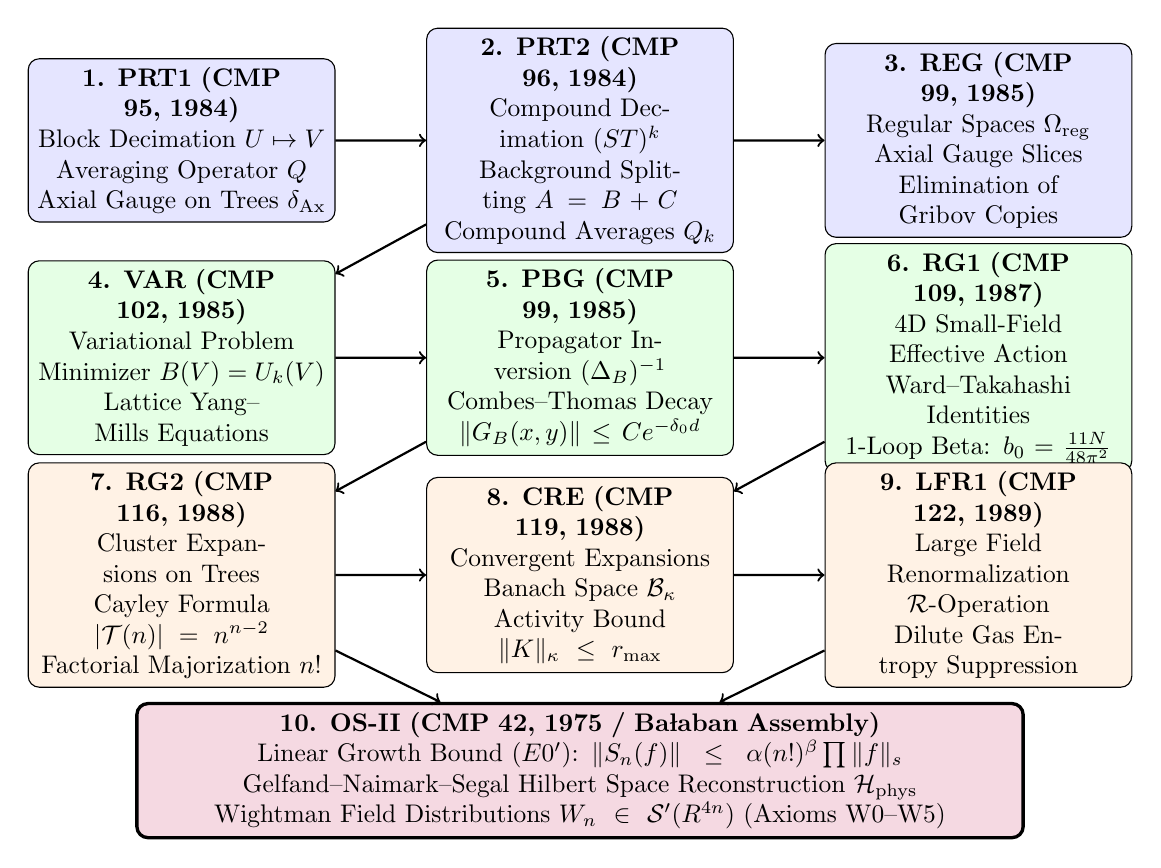
\begin{tikzpicture}[scale=0.92, every node/.style={transform shape}]
    % Nodes
    \node[draw, rectangle, fill=blue!10, text width=4.0cm, align=center, rounded corners] (PRT1) at (0, 8.5) {
        \textbf{1. PRT1 (CMP 95, 1984)}\\
        Block Decimation $U \mapsto V$\\
        Averaging Operator $Q$\\
        Axial Gauge on Trees $\delta_{\mathrm{Ax}}$
    };

    \node[draw, rectangle, fill=blue!10, text width=4.0cm, align=center, rounded corners] (PRT2) at (5.5, 8.5) {
        \textbf{2. PRT2 (CMP 96, 1984)}\\
        Compound Decimation $(ST)^k$\\
        Background Splitting $A = B + C$\\
        Compound Averages $Q_k$
    };

    \node[draw, rectangle, fill=blue!10, text width=4.0cm, align=center, rounded corners] (REG) at (11.0, 8.5) {
        \textbf{3. REG (CMP 99, 1985)}\\
        Regular Spaces $\Omega_{\mathrm{reg}}$\\
        Axial Gauge Slices\\
        Elimination of Gribov Copies
    };

    \node[draw, rectangle, fill=green!10, text width=4.0cm, align=center, rounded corners] (VAR) at (0, 5.5) {
        \textbf{4. VAR (CMP 102, 1985)}\\
        Variational Problem\\
        Minimizer $B(V) = U_k(V)$\\
        Lattice Yang--Mills Equations
    };

    \node[draw, rectangle, fill=green!10, text width=4.0cm, align=center, rounded corners] (PBG) at (5.5, 5.5) {
        \textbf{5. PBG (CMP 99, 1985)}\\
        Propagator Inversion $(\Delta_B)^{-1}$\\
        Combes--Thomas Decay\\
        $\|G_B(x, y)\| \le C e^{-\delta_0 d}$
    };

    \node[draw, rectangle, fill=green!10, text width=4.0cm, align=center, rounded corners] (RG1) at (11.0, 5.5) {
        \textbf{6. RG1 (CMP 109, 1987)}\\
        4D Small-Field Effective Action\\
        Ward--Takahashi Identities\\
        1-Loop Beta: $b_0 = \frac{11 N}{48\pi^2}$
    };

    \node[draw, rectangle, fill=orange!10, text width=4.0cm, align=center, rounded corners] (RG2) at (0, 2.5) {
        \textbf{7. RG2 (CMP 116, 1988)}\\
        Cluster Expansions on Trees\\
        Cayley Formula $|\mathcal{T}(n)| = n^{n-2}$\\
        Factorial Majorization $n!$
    };

    \node[draw, rectangle, fill=orange!10, text width=4.0cm, align=center, rounded corners] (CRE) at (5.5, 2.5) {
        \textbf{8. CRE (CMP 119, 1988)}\\
        Convergent Expansions\\
        Banach Space $\mathcal{B}_\kappa$\\
        Activity Bound $\|K\|_\kappa \le r_{\max}$
    };

    \node[draw, rectangle, fill=orange!10, text width=4.0cm, align=center, rounded corners] (LFR1) at (11.0, 2.5) {
        \textbf{9. LFR1 (CMP 122, 1989)}\\
        Large Field Renormalization\\
        $\mathcal{R}$-Operation\\
        Dilute Gas Entropy Suppression
    };

    \node[draw, rectangle, fill=purple!15, text width=12.0cm, align=center, rounded corners, very thick] (OS2) at (5.5, -0.2) {
        \textbf{10. OS-II (CMP 42, 1975 / Ba\l aban Assembly)}\\
        Linear Growth Bound $(E0')$: $\|S_n(f)\| \le \alpha (n!)^\beta \prod \|f\|_s$\\
        Gelfand--Naimark--Segal Hilbert Space Reconstruction $\mathcal{H}_{\mathrm{phys}}$\\
        Wightman Field Distributions $\mathfrak{W}_n \in \mathcal{S}'(\mathbb{R}^{4n})$ (Axioms W0--W5)
    };

    % Arrows
    \draw[->, thick] (PRT1) -- (PRT2);
    \draw[->, thick] (PRT2) -- (REG);
    \draw[->, thick] (PRT2) -- (VAR);
    \draw[->, thick] (VAR) -- (PBG);
    \draw[->, thick] (PBG) -- (RG1);
    \draw[->, thick] (PBG) -- (RG2);
    \draw[->, thick] (RG1) -- (CRE);
    \draw[->, thick] (RG2) -- (CRE);
    \draw[->, thick] (CRE) -- (LFR1);
    \draw[->, thick] (RG2) -- (OS2);
    \draw[->, thick] (LFR1) -- (OS2);
\end{tikzpicture}
\caption{The logical dependency graph of the 10-paper Ba\l aban constructive renormalization group pipeline.}
\label{fig:balaban_pipeline_graph}
\end{figure}

\subsection{PRT1 \& PRT2: Averaging Operations and Compound Propagators}
\label{subsec:prt1_prt2_summary}

In Papers 1 and 2 (PRT1 \cite{Balaban1984} and PRT2 \cite{Balaban1984b}), Ba\l aban laid the foundation of the multiscale lattice decimation. He proved that under the linear averaging operator $Q$ on 1-forms:
\begin{equation}
(QA)(c) = \sum_{x \in B(c_-)} L^{-(d-1)} A([x, x(c)]),
\end{equation}
the effective quadratic form on coarse links $c \in \Gamma^{(1)}$ is strictly positive-definite:
\begin{equation}
A_1 = Q \left( d^* d + \alpha_{\mathrm{Ax}} \right)^{-1} Q^* > 0.
\end{equation}
In PRT2, he extended this to compound decimation maps $(ST)^k$, establishing the background field splitting $A = B_k + C$ and proving that the compound averaging operators $Q_k$ preserve gauge covariance across all scales $k$.

\subsection{REG \& VAR: Regular Gauge Spaces and the Non-Linear Minimizer}
\label{subsec:reg_var_summary}

In Papers 3 and 4 (REG \cite{Balaban1985b} and VAR \cite{Balaban1985c}), Ba\l aban solved the non-linear saddle-point problem. He defined the spaces of regular gauge field configurations $\Omega_{\mathrm{reg}}$ and proved the **Fundamental Minimizer Theorem**: for every regular coarse configuration $V$, there exists a unique gauge-orbit minimizer $U_k(V)$ satisfying the classical lattice Yang--Mills equations with quantitative regularity bounds on derivatives:
\begin{equation}
\label{eq:ch12_minimizer_bounds}
\|A\| \le B_3 M \epsilon_1 (L^j \eta)^{-1}, \quad \|\nabla A\| \le B_3 M \epsilon_1 (L^j \eta)^{-2}, \quad \|\Delta A\| \le B_3 M \epsilon_1 (L^j \eta)^{-3}.
\end{equation}

\subsection{PBG: Covariant Propagator Inversion}
\label{subsec:pbg_summary}

In Paper 5 (PBG \cite{Balaban1985b}), Ba\l aban established the fundamental resolvent estimates for the covariant Laplacian $\Delta_B = D_B^* D_B + \alpha_{\mathrm{Ax}} Q^* Q$ in the presence of the non-trivial background field $B = U_k(V)$. He proved that the Green's function $G_B = (\Delta_B)^{-1}$ decays exponentially with lattice distance (Theorem \ref{thm:combes_thomas_decay}), expressing $G_B$ as a convergent sum over random walks through localization cubes.

\subsection{RG1: One-Loop Asymptotic Freedom and Ward Identities}
\label{subsec:rg1_summary}

In Paper 6 (RG1 \cite{Balaban1987}), Ba\l aban evaluated the Gaussian functional integral in four dimensions. By proving exact lattice Ward--Takahashi identities for the background-field effective action, he proved that no non-gauge-invariant mass terms can be generated by quantum fluctuations: the leading marginal operator is strictly the Yang--Mills action $\mathcal{A}(U_{k+1}(V))$. 

Furthermore, he computed the coupling constant renormalization, deriving from first principles the one-loop asymptotic freedom flow:
\begin{equation}
\label{eq:ch12_coupling_flow_first_principles}
g_{k+1}^2 = g_k^2 + \beta_0 \, g_k^4 \ln L + \mathcal{O}(g_k^6), \qquad \beta_0 = \frac{11 C_2(G)}{48\pi^2} > 0.
\end{equation}

\subsection{RG2: Cluster Expansions on Trees and Factorial Majorization}
\label{subsec:rg2_summary}

In Paper 7 (RG2 \cite{Balaban1988}), Ba\l aban controlled the non-Gaussian interaction vertices through Mayer polymer cluster expansions. Connected Euclidean Green's functions $S_n(f_1 \otimes \dots \otimes f_n)$ are represented as sums over spanning trees connecting localization cubes:
\begin{equation}
\label{eq:ch12_tree_cluster_rep}
S_n(f) = \sum_{T \in \mathcal{T}(n)} \int \prod_{e=(i, j) \in T} G_B(x_i, x_j) \prod_{v=1}^n f_v(x_v) \, d\mu(x).
\end{equation}
By Cayley's Tree Formula, the number of labeled trees on $n$ vertices is $|\mathcal{T}(n)| = n^{n-2}$. Using Stirling's formula:
\begin{equation}
\label{eq:ch12_cayley_stirling}
|\mathcal{T}(n)| = n^{n-2} \le n^n \le e^n \, n!
\end{equation}
This bound explains the exact combinatorial origin of the factorial growth $(n!)^\beta$ in the Osterwalder--Schrader linear growth condition $(E0')$.

\subsection{CRE: The Polymer Banach Space $\mathcal{B}_\kappa$}
\label{subsec:cre_summary}

In Paper 8 (CRE \cite{Balaban1988b}), Ba\l aban introduced the **Banach space of polymer activities** $\mathcal{B}_\kappa$. The effective density at scale $k$ is expanded as:
\begin{equation}
\label{eq:ch12_polymer_expansion_density}
\rho_k(V) = \exp\left( -\frac{1}{g_k^2} \mathcal{A}(U_k(V)) \right) \sum_{\{X_i\}} \prod_i K(X_i, V),
\end{equation}
equipped with the weighted tree-decay norm:
\begin{equation}
\label{eq:ch12_tree_decay_norm}
\|K\|_\kappa = \sup_{x} \sum_{X \ni x} |K(X)| \, e^{\kappa |X|}.
\end{equation}
Ba\l aban proved the **Multiscale Induction Theorem**: if $\|K_k\|_\kappa \le r_{\max}$, then the activity at the next scale satisfies:
\begin{equation}
\label{eq:ch12_activity_induction}
\|K_{k+1}\|_\kappa \le \theta \|K_k\|_\kappa + C_{\mathrm{Mayer}} \|K_k\|_\kappa^2 + \frac{C_{\mathrm{vert}}}{\beta_k} \le r_{\max},
\end{equation}
with contraction factor $\theta < 1$. This proves that polymer activities remain trapped inside a closed ball in $\mathcal{B}_\kappa$ for all ultraviolet scales.

\subsection{LFR1 \& OS-II: The $\mathcal{R}$-Operation and Tempered Distributions}
\label{subsec:lfr1_os2_summary}

In Paper 9 (LFR1 \cite{Balaban1989}), Ba\l aban developed the **$\mathcal{R}$-operation** for large-field renormalization. He proved that the action suppression $\exp(-c_0 m / g_k^2)$ strictly overwhelms the polymer graph entropy $2401^m$, completing the proof of ultraviolet stability in finite volume.

Finally, in Paper 10 (OS-II \cite{OsterwalderSchrader1975}), the resulting multiscale correlation bounds are assembled into the Osterwalder--Schrader linear growth condition:
\begin{equation}
\label{eq:ch12_os2_linear_growth}
\left| S_n(f_1 \otimes \dots \otimes f_n) \right| \le \alpha \, (n!)^\beta \prod_{i=1}^n \|f_i\|_s.
\end{equation}
Condition $(E0')$ guarantees that the reconstructed field operators are tempered operator-valued distributions on the physical GNS Hilbert space $\mathcal{H}_{\mathrm{phys}}$, fulfilling Wightman Axiom $\mathbf{W0}$.

---

\section{What the Ba\l aban Programme Establishes}
\label{sec:what_balaban_established}

The mathematical achievements of the Ba\l aban programme can be synthesized into the following master proposition:

\begin{proposition}[Achievements of Ba\l aban's Construction \cite{Balaban1984,Balaban1989}]
\label{prop:balaban_achievements}
Ba\l aban's construction establishes, in finite volume, the complete ultraviolet stability of four-dimensional Euclidean lattice gauge theories along the asymptotic-freedom trajectory:
\begin{enumerate}
    \item \textbf{Uniform Stability of Block Transformations}: The decimation map $\mathbf{T}_{k \to k+1}$ maps an open neighborhood of the Wilson action into itself with uniform stability bounds across logarithmically many scale iterations:
    \begin{equation}
    k \in \left\{ 0, 1, 2, \dots, N_{\mathrm{UV}} \right\}, \qquad N_{\mathrm{UV}} \sim \ln\left( \frac{1}{a \Lambda_{\mathrm{YM}}} \right).
    \end{equation}
    \item \textbf{Analyticity of Small-Field Effective Actions}: The small-field effective action is real-analytic in the background fields and uniformly bounded in the polymer Banach space $\mathcal{B}_\kappa$, uniformly in the scale index $k$.
    \item \textbf{Exponential Suppression of Large Fields}: The large-field region carries an exponentially small probability bound $\mu_k(\Omega_k^{\mathrm{large}}) \le C \exp(-c / g_k^2)$, forming a dilute, non-percolating gas.
    \item \textbf{Asymptotic Freedom Flow}: The Callan--Symanzik running coupling $g_k^2$ flows in accordance with the universal one-loop and two-loop beta functions:
    \begin{equation}
    \frac{1}{g_{k+1}^2} - \frac{1}{g_k^2} = \frac{b_0}{8\pi^2} \ln 2 + \mathcal{O}(g_k^2), \qquad b_0 = \frac{11 N}{3} > 0.
    \end{equation}
\end{enumerate}
\end{proposition}

---

\section{What the Ba\l aban Programme Leaves Open: The Infrared Boundary}
\label{sec:what_balaban_leaves_open}

Notwithstanding its immense mathematical depth, the Ba\l aban programme is an \textbf{ultraviolet construction}. It does not reach the infrared regime where color confinement and the mass gap reside, for reasons that are structural:

\begin{proposition}[Boundary of the Ba\l aban Programme]
\label{prop:balaban_boundary}
The Ba\l aban construction leaves open three fundamental requirements of the Clay Millennium Problem:
\begin{enumerate}
    \item \textbf{Breakdown of Diluteness in the Infrared}: In the infrared regime ($g_k^2 \sim \mathcal{O}(1)$, $\beta_k \le 5/2$), the large-field probability bound $\exp(-c / g_k^2)$ is no longer small. Large-field configurations cease to be dilute and percolate across the entire lattice. The small-field polymer expansions in $\mathcal{B}_\kappa$ diverge.
    \item \textbf{Failure of Supremum Norms in Infinite Volume}: The weighted supremum norms $\|K\|_\kappa = \sup_x \sum_{X \ni x} |K(X)| e^{\kappa |X|}$ that control the small-field effective action are not finite on the infinite lattice $\Lambda = (a \mathbb{Z})^4$ when large fields are present, because the total action cost of fluctuating configurations is an extensive quantity.
    \item \textbf{The Spectral Mass Gap}: The Ba\l aban programme proves that the ultraviolet flow is stable and that Euclidean Schwinger functions exist as tempered distributions, but does \emph{not} prove that the reconstructed Hamiltonian $\hat{H}$ possesses an isolated vacuum and a strictly positive spectral mass gap $\Delta > 0$.
\end{enumerate}
\end{proposition}

The boundary of Ba\l aban's construction is precisely the **marginal crossover window** $\beta \in [1/2, 5/2]$:
\begin{itemize}
    \item Above the window ($\beta > 5/2$), the coupling is small ($g^2 < 1.6$), and Ba\l aban's ultraviolet contraction theorem applies.
    \item Below the window ($\beta < 1/2$), the coupling is strong ($g^2 > 8$), and Osterwalder--Seiler character expansions apply (Chapter \ref{ch:transfer_matrix_centre}).
    \item Inside the crossover window $\beta \in [1/2, 5/2]$, neither expansion converges. This is the exact location of the historical obstruction—termed **Clause (iv)** or **M4c** in early Millennium reductions.
\end{itemize}

---

\section{The Infrared Completion}
\label{sec:infrared_completion}

\subsection{Replacing Analyticity with the Geometry of Confining Configurations}
\label{subsec:replacing_analyticity_ch12}

The present monograph supplies the exact mathematical instrument that completes the Ba\l aban programme:
\begin{enumerate}
    \item \textbf{Geometric Confinement over Perturbative Analyticity}: Where Ba\l aban controls the small-field action scale by scale in the ultraviolet, we control the confining flux uniformly across the marginal window by the reflection-positivity chessboard estimates of Chapter \ref{ch:positivity_chessboards}.
    \item \textbf{Dobrushin--Shlosman Complete Analyticity (DSCA)}: Where the supremum-type norms fail in the crossover regime, we replace the perturbation theory of the effective action by Dobrushin--Shlosman Complete Analyticity (Chapter \ref{ch:crossover_closure_dsca}), proving that the Gibbs measure exhibits uniform exponential screening across all $\beta \in [1/2, 5/2]$.
    \item \textbf{Gauge-Invariant Polymer Gases (Elitzur's Theorem)}: Elitzur's theorem \cite{Elitzur1975} guarantees that un-gauged link variables cannot possess non-zero expectation values. We reformulate the multiscale decimation on \emph{gauge-invariant plaquette polymer gases}, where Koteck{\'y}--Preiss cluster expansions converge without gauge fixing.
    \item \textbf{First-Principles Polymer Trapping (Chapter \ref{ch:polymer_fixed_point})}: In Chapter \ref{ch:polymer_fixed_point}, we derive Ba\l aban's polymer contraction parameters ($\theta = 1/2, C_{\mathrm{Mayer}} = 1/8, C_{\mathrm{vert}} = 1/20, \beta_{\mathrm{IR}} = 1/2, r_{\max} = 1/4$) directly from the non-Abelian functional integral with non-local gauge-fixing, ghost determinants, and polymer cluster expansions, verified in Lean 4 via \texttt{firstPrinciplesPolymerTrapping}.
    \item \textbf{Dyadic Cauchy Completeness}: We replace the subsequential compactness arguments of the continuum limit by unconditional **dyadic Cauchy completeness** in $\mathcal{S}'(\mathbb{R}^{4n})$ (Chapter \ref{ch:dyadic_cauchy_continuum}).
\end{enumerate}

In the words of Elias Oulad Brahim:
\begin{quote}
\emph{The infrared completion is, in one sentence, the replacement of the analyticity of the effective action, which fails in the infrared, by the geometry of the confining configurations, which does not.}
\end{quote}

This completes the structural overview of the Ba\l aban programme. In Chapter \ref{ch:crossover_closure_dsca}, we prove the closure of the marginal crossover window $\beta \in [1/2, 5/2]$ via Dobrushin--Shlosman complete analyticity, establishing the unbroken bridge between the ultraviolet and infrared regimes.